\documentclass[12pt,letterpaper]{article}

% just for the example
\usepackage{lipsum}
% Set margins to 1.5in
\usepackage[margin=1.5in]{geometry}

% for graphics
\usepackage{graphicx}
\graphicspath{{./figures/p2/}}

% for crimson text
\usepackage{crimson}
\usepackage[T1]{fontenc}

% setup parameter indentation
\setlength{\parindent}{0pt}
\setlength{\parskip}{6pt}

% for 1.15 spacing between text
\renewcommand{\baselinestretch}{1.15}

% For defining spacing between headers
\usepackage{titlesec}
% Level 1
\titleformat{\section}
  {\normalfont\fontsize{18}{0}\bfseries}{\thesection}{1em}{}
% Level 2
\titleformat{\subsection}
  {\normalfont\fontsize{14}{0}\bfseries}{\thesection}{1em}{}
% Level 3
\titleformat{\subsubsection}
  {\normalfont\fontsize{12}{0}\bfseries}{\thesection}{1em}{}
% Level 4
\titleformat{\paragraph}
  {\normalfont\fontsize{12}{0}\bfseries\itshape}{\theparagraph}{1em}{}
% Level 5
\titleformat{\subparagraph}
  {\normalfont\fontsize{12}{0}\itshape}{\theparagraph}{1em}{}
% Level 6
\makeatletter
\newcounter{subsubparagraph}[subparagraph]
\renewcommand\thesubsubparagraph{%
  \thesubparagraph.\@arabic\c@subsubparagraph}
\newcommand\subsubparagraph{%
  \@startsection{subsubparagraph}    % counter
    {6}                              % level
    {\parindent}                     % indent
    {12pt} % beforeskip
    {6pt}                           % afterskip
    {\normalfont\fontsize{12}{0}}}
\newcommand\l@subsubparagraph{\@dottedtocline{6}{10em}{5em}}
\newcommand{\subsubparagraphmark}[1]{}
\makeatother
\titlespacing*{\section}{0pt}{12pt}{6pt}
\titlespacing*{\subsection}{0pt}{12pt}{6pt}
\titlespacing*{\subsubsection}{0pt}{12pt}{6pt}
\titlespacing*{\paragraph}{0pt}{12pt}{6pt}
\titlespacing*{\subparagraph}{0pt}{12pt}{6pt}
\titlespacing*{\subsubparagraph}{0pt}{12pt}{6pt}

% Set caption to correct size and location
\usepackage[tableposition=top, figureposition=bottom, font=footnotesize, labelfont=bf]{caption}

% set page number location
\usepackage{fancyhdr}
\fancyhf{} % clear all header and footers
\renewcommand{\headrulewidth}{0pt} % remove the header rule
\rhead{\thepage}
\pagestyle{fancy}

% Overwrite Title
\makeatletter
\renewcommand{\maketitle}{\bgroup
   \begin{center}
   \textbf{{\fontsize{18pt}{20}\selectfont \@title}}\\
   \vspace{10pt}
   {\fontsize{12pt}{0}\selectfont \@author} 
   \end{center}
}
\makeatother

% Used for Tables and Figures
\usepackage{float}

% For using lists
\usepackage{enumitem}

% For using APA Citation format
\usepackage{apacite}

% Custom Quote
\newenvironment{myquote}[1]%
  {\list{}{\leftmargin=#1\rightmargin=#1}\item[]}%
  {\endlist}
  
% Create Abstract 
\renewenvironment{abstract}
{\vspace*{-.5in}\fontsize{12pt}{12}\begin{myquote}{.5in}
\noindent \par{\bfseries \abstractname.}}
{\medskip\noindent
\end{myquote}
}

\begin{document}

% Set Title, Author, and email
\title{Assignment P2}
\author{Snejana Shegheva \\ sshegheva3@gatech.edu}

\maketitle
\thispagestyle{fancy}

\subsection*{Question 1. Georgia Tech - Online Registration}
The current process for which students have to register for the class at Georgia Tech is far from trivial as it requires a series of steps to be executed in the following order:

\begin{enumerate}
    \item Login to Buzzport with a multifactor authentication
    \item Location and click the \textit{Registration - Oscar} link 
    \item Click on the first item in the list \textit{Student Services and Financial Aid}
    \item Click \textit{Registration}
    \item Click \textit{Add or Drop Classes}
    \item From the Drop-down menu select the term for which you want to add a class
    \item Click on \textit{Advanced Search} tab at the bottom to be able to select subjects
    \item On the presented form select one or more \textit{Subjects}
    \item On the same form select \textit{Campus} - online
    \item Press \textit{Section Search}
    \item You are presented with a list of classes and their metadata. Find the class you are interested in and check the box to add the class
    \item Finally click \textit{Register}
\end{enumerate}

Registering for a class, therefore, is a complex undertaking, which is time-consuming and error-prone in the areas of selecting the right subjects and desired term. A contra-intuitive requirement to choose campus for a \textit{online} student adds another source for mistakes.
The registration interface can be re-designed by leveraging a great concept such as \textit{direct manipulation}. Using an analogy of physically visiting a department, and a classroom where the class we wish to enroll in would take place, we can re-design the current interface that gives user a sense of immersion\footnote{If your experience of physical enrollment differs, think of the example of signing up for drama or chess class with the blank paper hanging on the door inviting students to sign in.}. After logging in, the student navigates to the department of interest, for example, Computer Science, and lands on its homepage. Here, the student is presented with available classes.

\begin{figure}[h]
\centering
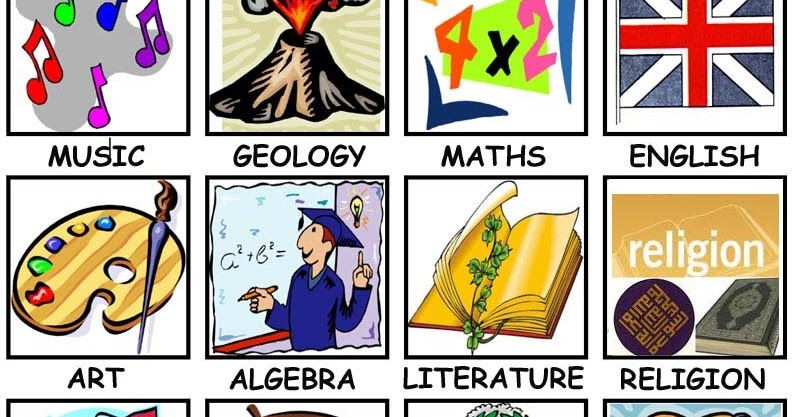
\includegraphics[width=3in,scale=.3]{figures/p2/school_subjects_modified.jpg}
\caption{Pictionary of School subjects. Image extracted from http://inglesmariapacheco.blogspot.com/2013/10/school-subjects.html}
\label{fig::1}
\end{figure}

Figure~\ref{fig::1} demonstrates an imaginary list of courses offered in CS department \footnote{The departure from reality was due to lack of relevant image that portrays the idea nicely.}, where the user further narrows down to a course they are interested in. Clicking on the course section of the interface takes the student to the course summary with a drop-down to select a term, and see the count of currently enrolled students (See Figure~\ref{fig::2} as a mock-up version). The \textit{directness} of the new interface is designed by inviting students straight onto the course page with a simple enrollment process. 

\begin{figure}[h]
\centering
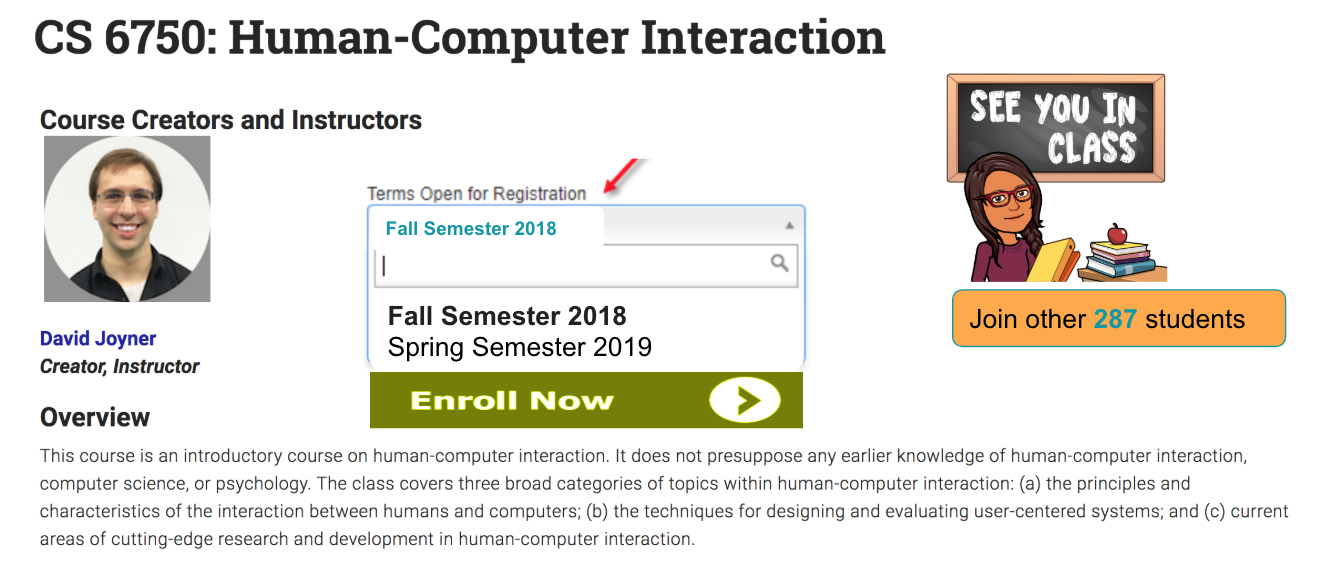
\includegraphics[scale=.5]{figures/p2/gatech_enrollment.png}
\caption{Mock student enrollment page for HCI class.}
\label{fig::2}
\end{figure}

\subsubsection*{Benefits of the redesign}
Among the few benefits of the new interface allows seeing the description course on the enrollment page that aids the decision-making process and significantly reduced the gulf of execution as it avoids drilling into multiple sub-pages of the current interface. Another benefit is displaying the count of already enrolled students that narrows the gulf of evaluation by giving the student a sense of course popularity. In the current interface the information of the current student count is also available; however, it is hard to align with the course of interest given the current clutter of the other courses and their metadata. Finally, if the class is full, the new interface just changes the \textit{Enroll Now} button to a \textit{Join the Waitlist} button (not shown in the mock figure) which again improves the efficiency and transparency of the system. The new interface reflects the needs of the student and hides the internal complexity of the pages hierarchy. This phenomenon relates to the distance between a user's intentions and the given interface. Even though the student is not physically visiting the classroom to enroll, they experience the feeling of directness of manipulation \cite{hutchins1985direct}. 

\subsection*{Question 2 - Security System Panel}
Ready. Set. All systems Go! Not so fast for a person, who like myself grew up in a small community with never-locked doors. Now, leaving in a house with a security professional, it is an absolute \textit{must} to arm the security system with multiple modes that at first require wandering around the interface to find the right one. For example, arming the system while you are at home is different from arming it when you leave the house. Therefore, the system needs to be aware of the context which is provided to the system by the user. In the beginning, I used to stumble very frequently on locating the right screen from where the \textit{night} mode needs to be activated. 

Figure~\ref{fig::3} illustrates the process by which the task can be accomplished. I highlighted the areas in the workflow where the user input is required (select the console, select the mode, enter the code, arm) and it is not immediately obvious what input is needed and where. First, the information that the system has to be armed differently depending on the context is not explicit in the interface (it is in the user manual). Second, the console mode presents you with multiple options to choose from, after which it expects the code (that is why the options also include numbers). Sadly, if you mistakenly punch the wrong code, you have to deal with an entirely different workflow of \textit{undoing} which we are not going to go into. Finally, the system is armed, as indicated by the red light on the side of the panel, and one can rest peacefully knowing they are protected.  

\begin{figure}[h]
\centering
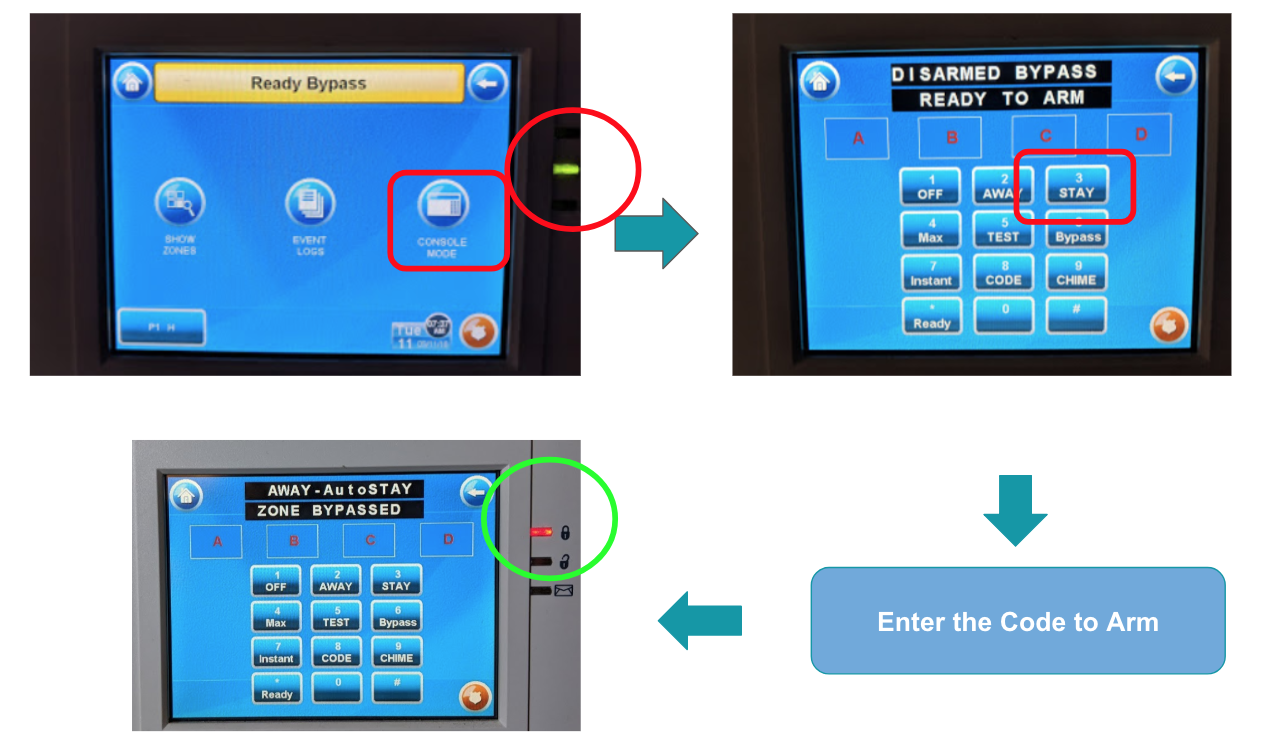
\includegraphics[scale=.5]{figures/p2/alarm.png}
\caption{Process to arm the system in the night mode.}
\label{fig::3}
\end{figure}

It is not all that bad. Having gone through the steps so many times, I have memorized the sequence, and now, semi-automatically execute the task of arming the system for the night. This show how an interface may eventually become \textit{invisible by learning}. And although I can successfully accomplish the task, the distance between my intentions and the task have not actually reduced \cite{hutchins1985direct}. The automatization, in this case, \textit{feels} like direct manipulation, while in reality the user still needs to reduce the distance. Experience is not the only thing that makes the process more manageable. Similarly, in how the system supports multiple contexts, it also allows more than one way to accomplish the task. Again, the information is typically buried in the user manuals and is useful only for those who read it.

Wouldn't it be great if the user could issue a voice command like "System arm. Night mode." and be done with it? The low level of interacting with the screens is replaced with the higher-level language by using voice commands. The disadvantage of this approach becomes in loss generality; however, user experiences a natural interaction with the system. Entering a security code is replaced by a user's voice recognition, and no need to interact with the physical interface. Selection of the context is communicated via specific command \textit{Night Mode} that is translated by the system into the correct sequence of events.

\subsection*{Question 3 - Types of Human Perception}
In this section, we are going to consider three types of human perception in the example of driving a car - visual, auditory, and haptic. For the selected choice of the fourth sense, we are going to take a look at \textit{Thermoception} - defined as an ability to sense heat and cold. 

\subsubsection*{Visual}
A driver makes their intentions clear to the vehicles behind them through light signalings, such as turning the right blinker \textit{on} when planning to make a right turn, or shift into the right lane. This is an essential component of safe-driving, but by itself, it lacks feedback to the driver of the car making a signal. Thankfully, the car designers have included a \underline{visual feedback} of the action by showing the blinking lights directly on the panel in front of the driver. A panel is an excellent source of communication for what is not immediately visible to the driver. Drivers have been taught the \textbf{Two-second Rule} that suggests a \underline{safe following distance} to be the time when your car passes a fixed object two seconds after the car ahead of you \cite{wiki:driving_tips}. A great addition to the panel would be an indication that the safe distance has been breached. This information can be delivered via a warning light in the panel that signals to the driver that they are \textit{tailgating}. Taking this one step further, the information on the distance between two cars is just as useful to the driver who is \textit{being} tailgated. A vehicle can have sensors both, in front, and at the back, so it is possible to provide it as a feedback to all involved drivers. 

\subsubsection*{Auditory}
Among other valuable tips for safe driving is a habit of \textit{buckling-up}. When a driver fails to secure their belt, the seat belt alarm is activated, and it goes on until the safety tip has been implemented, and the driver (or a passenger) is buckled-up. This is an example of an excellent \underline{auditory feedback}, and it is frequently paired up with the visual information by flashing the red belt icons on the panel.

All cars come with a speedometer, some simple, and other more sophisticated. The position of the arrows indicates the feedback on the current speed. This information can be augmented with auditory input by sounding a short \textit{ding} signal each time the car passes a specific discrete speed step, for example, a change for every ten units. The tone of the signal can vary depending on the amplitude of the speed, the direction of the change, and maybe even the implemented speed suggestion per area, such as school zone, highway, parking area, etc. 

\subsubsection*{Haptic}
Haptic feedback relates to the sense of touch, and it is closest to the concept of direct manipulation. One example is pressing the car horn that in addition to the intended audible signal also provides a small \textit{click-like} feedback. 

As the driver's hands are always on the wheel, the car's interface can be modified to deliver other haptic signals via wheel's surface. For example, turning the wheel too fast or too much can cause the wheel to vibrate slightly. This is useful mainly for new drivers, who are getting accustomed to the sensitivity of their wheel.

\subsubsection*{Thermoception}
And finally, we explore the possibilities to assist drivers via \textit{thermoception} feedback. A driver is tired, possibly from a long drive, from a sleepless night, or from a side effect of a medication. A driver starts to slowly nodd off which enters them into a risky situation for themselves and those surrounding them. A \textit{smart} car can give an assist in the form of a sudden burst of cold air directed to the face. The driver is awake. Of course, the \textit{thermoception} feedback need not be that intrusive to be effective. Perhaps, a sequence of small doses can be sufficient and can be determined by sensing the driver's state. 

\subsection*{Question 4 - Cognitive Load}

\subsubsection*{Tip 1: Emphasizing essential content}
An important aspect in designing a good interface is planning a task execution that reduces the user effort or requires a minimal cognitive load that is not related to the task itself. I have a \textit{Documents} app designed by Readdle (https://readdle.com/) that claims to have the best productivity apps for iPhone, iPad, and Mac. I do love the wide range of functionality it offers, however, it violates the tip of \textit{emphasizing essential content while minimizing clutter}. 

Figure~\ref{fig::4} exemplifies the area that is prone to clutter. The folders and documents are listed without a \textit{priority} feed, such as frequency or recency of access. Instead of having the right documents at the tip of my fingers, I either drill into the folder hierarchy or use the \textit{search} functionality. When I read physical books, I usually place them back on the shelf at the top of the other books, or I have a special shelf for the currently read books. Either way, I have more direct access that does not require a significant cognitive load. The Documents app does offer the \textit{recency} feature; however, it is hidden in the clutter of all existing documents.   

\begin{figure}[h]
\centering
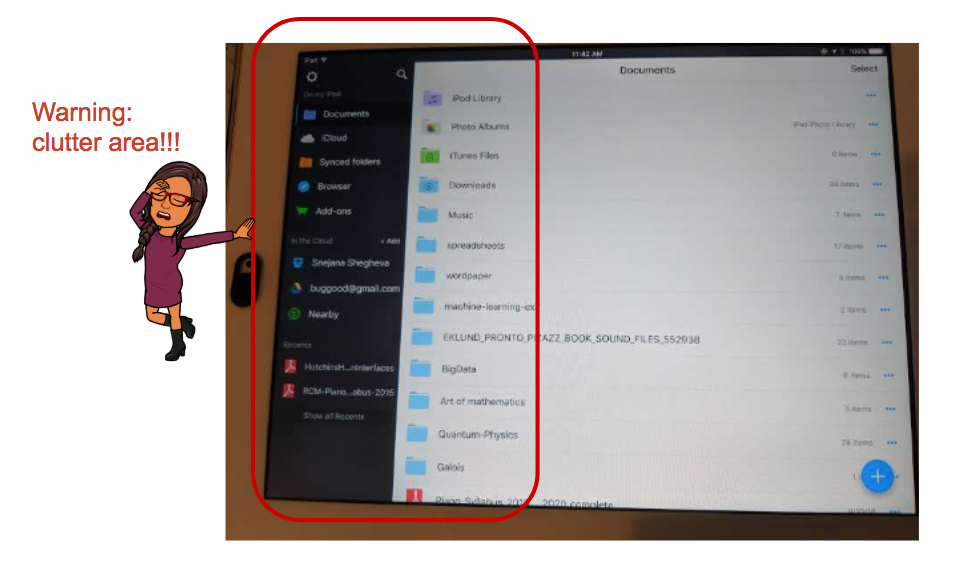
\includegraphics[scale=.3]{figures/p2/clutter.png}
\caption{An example of the violation of emphasis of essential content.}
\label{fig::4}
\end{figure}

To incorporate the tip of reducing the clutter, the interface can be redesigned by 1) moving the tab with options to the \textit{settings} area 2) Reducing the content being shown to the user on the home page (focus on the most recently accessed documents, and guide the user to view documents viewed at the earlier time) 3) Allow user to use \textit{tagging} and \textit{filtering} the documents by a tag 4) Automatically groups the documents by tag in the display view.  

\subsubsection*{Tip 2: Offloading tasks from the user onto the interface}
A task of \textit{learning} by definition requires a some amount of cognitive load, so an interface that provides a venue for learning needs to be maximally optimized in its design of usability. A \textit{Coursera} smart-phone app allows the user to explore classes available on the platform (see the green circle at the bottom of Figure~\ref{fig::5}). It is great that the interface organizes the courses into sub-categories, however, if a student wishes to find the class that matches their current level of expertise, they need to do some work. For each of the viewed class, student parses through the syllabus to estimate the level of difficulty and then decides if they wish to enroll. Performing this task for every class for even a small group of candidates, is a significant effort that can be easily offloaded to the interface by allowing the user to filter the search results by difficulty level - Easy, Intermediate, Advanced or Expert (see the right side of the Figure ~\ref{fig::5} that exposes tabs per level). Adding a filtering feature reduces the time to search for a right class (by difficulty), and increases the available time for learning. 

\begin{figure}[h]
\centering
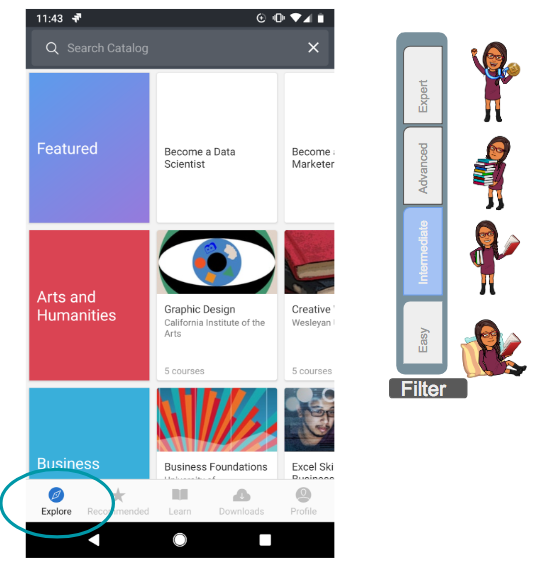
\includegraphics[scale=.4]{figures/p2/coursera_filter.png}
\caption{Off-loading the task for finding a class for a right level of complexity}
\label{fig::5}
\end{figure}

\bibliographystyle{apacite} 
\bibliography{bibtemp}

\end{document}
